\documentclass[11pt]{article}
\usepackage[T1]{fontenc}
\usepackage[utf8]{inputenc}
\usepackage{lmodern,amsmath,amssymb,graphicx,geometry,microtype,setspace,booktabs,caption}
\usepackage[hidelinks]{hyperref}
\geometry{letterpaper,margin=1in}
\setlength{\parindent}{0pt}
\setlength{\parskip}{0.55em}
\setlength{\emergencystretch}{2em}
\captionsetup{labelfont=bf,font=small}
\renewcommand{\refname}{References}
\pagestyle{empty}
\renewcommand{\thefigure}{S\arabic{figure}}
\setcounter{figure}{5}
\begin{document}
\begin{figure}[!ht]\centering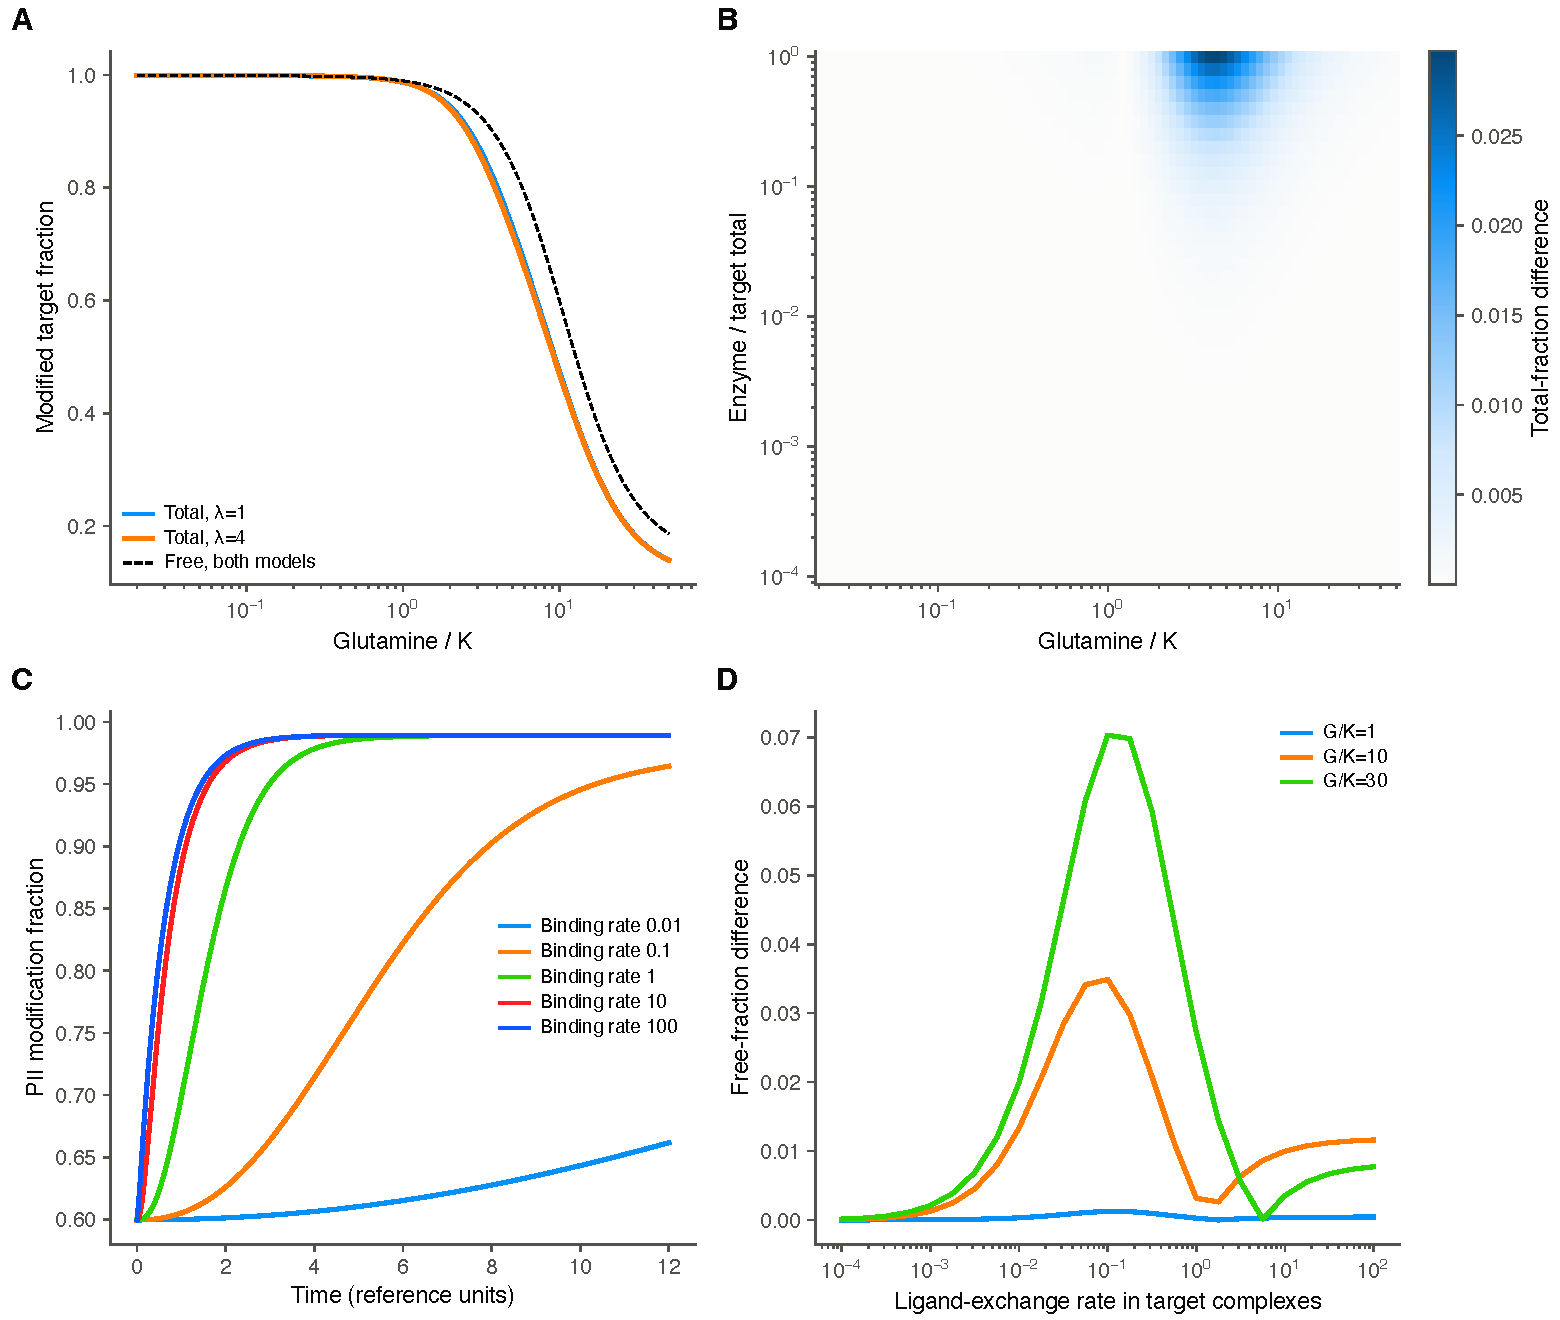
\includegraphics[width=\textwidth,height=0.60\textheight,keepaspectratio]{figure_inputs/FigS17_extended.pdf}\caption{\textbf{Reaction and observation assumptions define different boundaries.} (A) Explicit enzyme--target complexes preserve the free modified fraction but change total fractions; enzyme/target total is 0.3. (B) Total-fraction separation between $\lambda=1,4$ across enzyme/target ratios for one disclosed asymmetric-affinity scenario. Conservation bounds this separation by $\min(1,E_{\rm tot}/T_{\rm tot})$ in the stated monovalent model. (C) Finite regulatory binding changes the transient without changing its steady endpoint. Binding rates and time are dimensionless reference units. (D) Ligand exchange in substrate-bound complexes with state-dependent dissociation/catalysis ratios breaks free-state equivalence. This extension preserves thermodynamic binding-cycle ratios but permits catalytic regulatory currents. Its parameters and positive steady-state checks are specified in A8. All curves are calculations, not new observations.}
\end{figure}
\end{document}
